\documentclass[12pt,a4paper]{article}

% Packages
\usepackage{amsmath,amssymb}
\usepackage{graphicx}
\usepackage{tikz}
\usepackage{natbib}
\usepackage{geometry}
\geometry{margin=1in}

% Title
\title{The Principle of Emergent Cycles (PEC-E):\\
A Framework for Stability, Dissipation, and Emergence in Complex Systems}
\author{[Author Name]}
\date{\today}

\begin{document}

\maketitle

% Abstract
\begin{abstract}
We propose the \textbf{Principle of Emergent Cycles (PEC-E)}: in open, driven, non-equilibrium systems, dissipation explores numerous potential cyclic pathways, but only a rare subset achieves long-term persistence. This process, termed \emph{differential persistence}, acts as a pruning mechanism. Emergent cycles are those that occupy a viable region in a stability–dissipation trade-off space: they must sufficiently channel entropy (increasing the cycle-carried fraction $\phi$) while simultaneously enhancing the dynamic stability of the embedding system (e.g., shortening return times). This acquired stability, in turn, provides a reliable scaffold for higher-order organization. Instead of a single fitness score, we frame PEC-E in terms of a \emph{viability space} and outline a falsifiable, cross-disciplinary empirical program.
\end{abstract}

\section{Introduction}
Complex systems far from equilibrium exhibit striking emergent order: from chemical oscillations to biological cycles, ecosystems, and even socio-technical infrastructures. Existing principles such as Maximum Entropy Production or Constructal Law capture certain tendencies, but lack a unified mechanism for explaining how cycles emerge, persist, and scaffold higher-order structures. Here we propose the \emph{Principle of Emergent Cycles (PEC-E)}.

\section{Background}
Non-equilibrium thermodynamics has long acknowledged the role of dissipative structures (Prigogine), self-organization, and feedback in generating order. Network thermodynamics and stochastic thermodynamics formalize entropy production in terms of currents and affinities ($J_\alpha A_\alpha$). Yet a gap remains: why do certain recurrent loops persist while others vanish? PEC-E addresses this gap.

\section{Principle of Emergent Cycles (PEC-E)}

\subsection{Operational Definition}
A cycle $c$ is non-trivial if it exhibits positive entropy production at stationarity ($J_{\alpha} A_{\alpha} > 0$). A cycle is \emph{emergent} if it demonstrates \emph{differential persistence} by satisfying two primary conditions:
\begin{enumerate}
    \item \textbf{Increases channeled dissipation} $\Delta \phi(c) > 0$: the cycle organizes a significant fraction of the system’s total entropy production, moving the system away from purely linear dissipation.
    \item \textbf{Improves network stability} $\Delta \mathrm{Stab}(c) > 0$: the presence of the cycle enhances the stability of the larger network, measured by metrics such as shorter return times after perturbation, reduced variance of key observables, or an increased spectral gap.
\end{enumerate}

\subsection{The Viability Space and Emergent Set}
We reject the notion of a single, scalar ``fitness'' for a cycle. Instead, emergent cycles occupy a viable region within a multi-dimensional parameter space. For a given level of external \textbf{Drive} and internal \textbf{Feedback Richness}, a cycle’s persistence depends on its location in the space defined by $\phi$ (cycle-carried dissipation) and \textbf{Stability}.

As depicted in Figure~\ref{fig:viability}, this creates distinct regimes. At low drive or feedback, dissipation is predominantly linear. At high levels of both, a proliferation of unstable, interfering loops can lead to fragility or collapse. The emergent set
\[
E(C)
\]
consists of cycles in the ``green zone''—a region representing a sustainable trade-off where $\phi$ is sufficiently high without critically compromising stability. 

\emph{Composability}, the capacity to serve as a building block for new structures, is not a criterion for entry into this set but an \emph{outcome} of the stability it confers.

\begin{figure}[h]
\centering
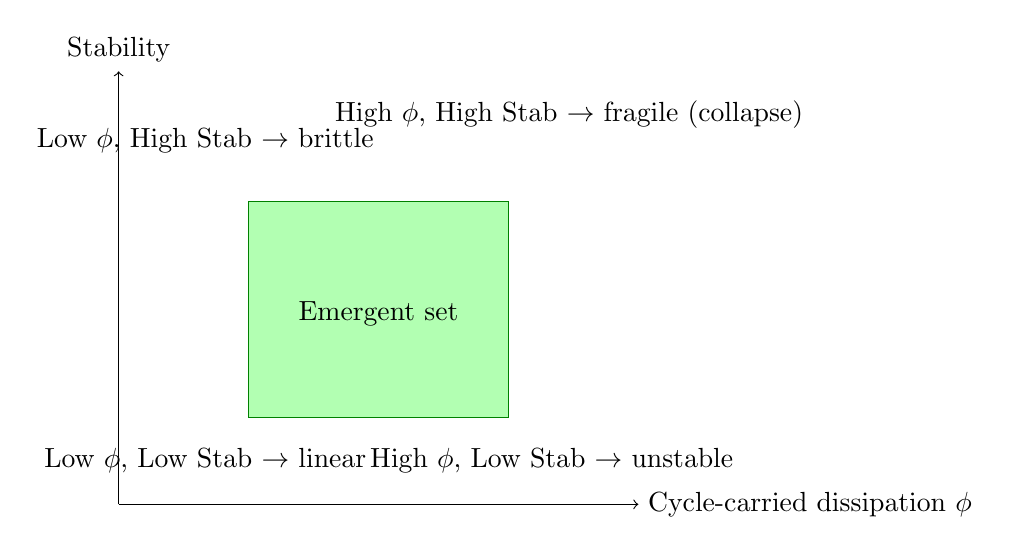
\begin{tikzpicture}[scale=1.1]
% Axes
\draw[->] (0,0) -- (6,0) node[right]{Cycle-carried dissipation $\phi$};
\draw[->] (0,0) -- (0,5) node[above]{Stability};

% Green zone
\fill[green!30,draw=green!50!black] (1.5,1) rectangle (4.5,3.5);
\node at (3,2.2) {Emergent set};

% Labels
\node at (5.2,4.5) {High $\phi$, High Stab $\to$ fragile (collapse)};
\node at (1,4.2) {Low $\phi$, High Stab $\to$ brittle};
\node at (5,0.5) {High $\phi$, Low Stab $\to$ unstable};
\node at (1,0.5) {Low $\phi$, Low Stab $\to$ linear};
\end{tikzpicture}
\caption{Schematic of the viability space showing the emergent set (green zone).}
\label{fig:viability}
\end{figure}

\subsection{Mechanism of Integration: Co-Creation and Wiggle}
While the viability space describes which cycles persist, it is equally important to articulate the micro-mechanism by which new elements become embedded into existing networks. We propose two complementary axioms: \emph{co-creation} and \emph{wiggle}.

\textbf{Co-creation.} A network generates the very conditions for its future members. Potential new configurations are themselves products of earlier cycles and constraints. Thus, every candidate element is partially shaped by the network’s history, architecture, and available degrees of freedom.

\textbf{Wiggle (reciprocal micro-adjustment).} Successful integration is never one-sided. Both the element and the existing network undergo small reciprocal adjustments—a ``wiggle.'' These adjustments preserve continuity while permitting novelty. The form of the wiggle depends on the nature and scale of the network:
\begin{itemize}
    \item Molecular: induced fit through conformational shifts in enzyme and ligand.
    \item Neural: synaptic weights adjust to incorporate new signals.
    \item Social: language, norms, or roles adapt incrementally to allow mutual fit.
\end{itemize}

Through co-creation and wiggle, networks maintain viability while exploring new configurations. In PEC-E, these processes provide the micro-dynamics by which cycles settle into the viable region, becoming stable and composable.

\section{Methodological Framework: Coarse-Graining and Measurement}
A rigorous application of PEC-E requires objective criteria for defining system states, as the calculation of $\phi$ depends on partitioning. We propose that partitions be justified by:
\begin{enumerate}
    \item \textbf{Functional boundaries} (e.g., membranes, species).
    \item \textbf{Timescale separation} (fast vs. slow variables).
    \item \textbf{Information-theoretic criteria} (maximizing predictive information).
\end{enumerate}

Future work must apply PEC-E to computational models to transparently test the sensitivity of $\phi$ across partitioning schemes.

\section{Case Studies}
To clarify applicability, we distinguish between:
\begin{itemize}
    \item \textbf{Type I (Self-Organized):} cycles emerge directly from dynamics.
    \item \textbf{Type II (Evolved/Encoded):} cycles are encoded by blueprints (e.g. genomes).
\end{itemize}

\subsection{Cellular Metabolism (Type II)}
The TCA cycle is a persistent loop encoded by evolution because it lies near the optimal viability region: high $\phi$ with stable homeostasis. Its composability is a consequence of stability.

\subsection{Ecosystems (Type I)}
Nutrient cycling after enrichment illustrates Type I emergence. Initial unstable predator-prey oscillations are pruned; persistent, weaker nutrient loops remain, enhancing system stability.

\section{Discussion}
PEC-E reframes emergence as \emph{differential persistence} in a viability space, rather than scalar fitness optimization. It integrates with existing principles (MaxEP, Constructal Law) by focusing on cycles as the structural units of dissipation and stability. Co-creation and wiggle provide the micro-mechanics of integration.

\section{Conclusion}
The Principle of Emergent Cycles offers a testable framework: cycles persist if they channel entropy while improving stability. This dual requirement explains why emergent loops scaffold higher-order organization. By grounding the theory in viability spaces, coarse-graining criteria, and case typologies, PEC-E establishes a rigorous and falsifiable research program across disciplines.

\bibliographystyle{plainnat}
\bibliography{refs}

\end{document}
